% --------------------------------------------------------------
% This is all preamble stuff that you don't have to worry about.
% Head down to where it says "Start here"
% --------------------------------------------------------------
 
\documentclass[12pt]{article}
 
\usepackage[margin=1in]{geometry} 
\usepackage{amsmath,amsthm,amssymb,scrextend}
\usepackage{fancyhdr}
\usepackage{enumitem}
\usepackage{amsmath}
\usepackage{amssymb}
\usepackage{textcomp}
\usepackage{fancybox}
\usepackage{tikz}
\usepackage{tasks}
\pagestyle{fancy}
\usepackage[makeroom]{cancel}
\usepackage{graphicx}
\usepackage{caption}
\usepackage{mwe}
\usepackage{tikz}
\usetikzlibrary{positioning}

\newcommand{\N}{\mathbb{N}}
\newcommand{\Z}{\mathbb{Z}}
\newcommand{\I}{\mathbb{I}}
\newcommand{\R}{\mathbb{R}}
\newcommand{\Q}{\mathbb{Q}}
\renewcommand{\qed}{\hfill$\blacksquare$}
\let\newproof\proof
\renewenvironment{proof}{\begin{addmargin}[1em]{0em}\begin{newproof}}{\end{newproof}\end{addmargin}\qed}
% \newcommand{\expl}[1]{\text{\hfill[#1]}$}
 
\newenvironment{theorem}[2][Theorem]{\begin{trivlist}
\item[\hskip \labelsep {\bfseries #1}\hskip \labelsep {\bfseries #2.}]}{\end{trivlist}}
\newenvironment{lemma}[2][Lemma]{\begin{trivlist}
\item[\hskip \labelsep {\bfseries #1}\hskip \labelsep {\bfseries #2.}]}{\end{trivlist}}
\newenvironment{problem}[2][Problem]{\begin{trivlist}
\item[\hskip \labelsep {\bfseries #1}\hskip \labelsep {\bfseries #2.}]}{\end{trivlist}}
\newenvironment{exercise}[2][Exercise]{\begin{trivlist}
\item[\hskip \labelsep {\bfseries #1}\hskip \labelsep {\bfseries #2.}]}{\end{trivlist}}
\newenvironment{reflection}[2][Reflection]{\begin{trivlist}
\item[\hskip \labelsep {\bfseries #1}\hskip \labelsep {\bfseries #2.}]}{\end{trivlist}}
\newenvironment{proposition}[2][Proposition]{\begin{trivlist}
\item[\hskip \labelsep {\bfseries #1}\hskip \labelsep {\bfseries #2.}]}{\end{trivlist}}
\newenvironment{corollary}[2][Corollary]{\begin{trivlist}
\item[\hskip \labelsep {\bfseries #1}\hskip \labelsep {\bfseries #2.}]}{\end{trivlist}}
 
\setlength{\parindent}{0pt}
\begin{document}
 \settasks{
	counter-format=(tsk[r]),
	label-width=4ex
}
% --------------------------------------------------------------
%                         Start here
% --------------------------------------------------------------

\lhead{Math 632}
\chead{Homework 6}
\rhead{Meenmo Kang}

\noindent
\textbf{1.} Let $\{N(t):t\ge 0\}$ be a rate $\lambda$ Poisson process, $\{T_k\}_{k\ge 1}$ the arrival times of the process, and $\tau_k = T_k - T_{k-1}$ for $k\ge 1$ the interarrival times. Calculate the probabilities below. When unspecified non-negative integers $j$ and/or $k$ appear in the question, your answer should cover all possible cases. When units are used, suppose the time unit is second.
\begin{enumerate}[label=(\alph*)]
    \item $P(N(2) = j,\; N(5)=k)$
    
    $$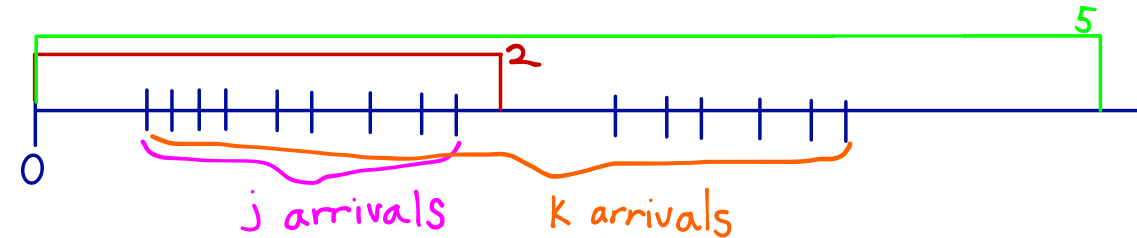
\includegraphics[height=1.4cm, width=12cm]{HW6/P1_1.jpeg}$$
    \begin{enumerate}[label=(\roman*)]
    
    \item $0<j\le k$
    $$P(N(2) = j)\cap P(N(5)=k)
    =P(N(2) = j)\cap P(N(5)-N(2)=k-j)
    $$
    $$   \left(e^{-2\lambda}\cdot \frac{(2\lambda)^j}{j!}\right)\cdot \left(e^{-3\lambda}\cdot \frac{(3\lambda)^{k-j}}{(k-j)!} \right) 
    = e^{-5\lambda}\cdot \frac{2^j3^{k-j}\lambda^k}{k!}   $$
    
    \item There is no probability in cases where $j>k$ or $j\le 0$.
    $$P(N(2) = j,\; N(5)=k)=
    \begin{cases}
    e^{-5\lambda}\cdot \frac{2^j3^{k-j}\lambda^k}{k!}  & \text{if } 0<j\le k\\
    0 & \text{if } j\le 0 \text{ or } j > k
    \end{cases}
    $$
    \end{enumerate}
    
    \item P(after the 3rd arrival there are no arrivals for 20 seconds,\\ 
    \qquad but after that the next two arrivals come within 10 seconds)
    $$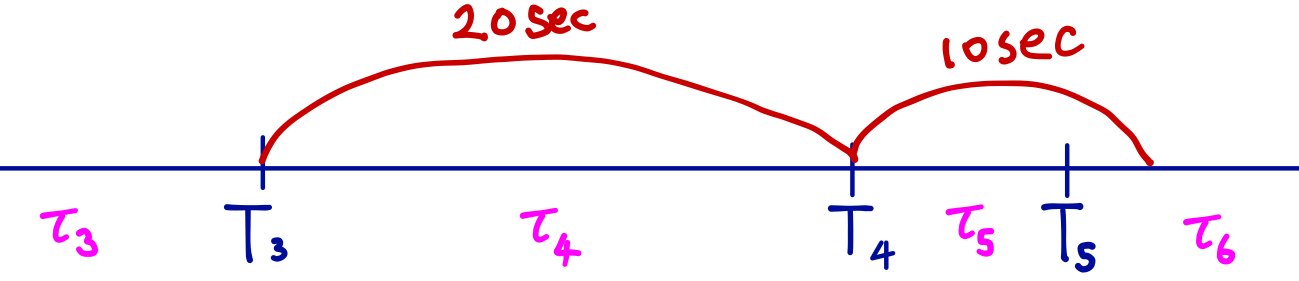
\includegraphics[height=1.4cm, width=12cm]{HW6/P1.jpeg}$$
    $$\text{No arrival for 20 seconds after $T_3$: }P(\tau_4 > 20) = P(N(20)=0) = e^{-20\lambda}\cdot \frac{(20\lambda)^0}{0!}=e^{-20\lambda}$$
    $$\text{Two arrivals within 10 seconds after $T_4$: }P(N(10)=2)= e^{-10\lambda}\cdot \frac{(10\lambda)^{2}}{2!}$$
    So the ultimate probability we are trying to get is
    $$e^{-20\lambda}\cdot e^{-10\lambda}\cdot \frac{(10\lambda)^2}{2!} = e^{-30\lambda}\cdot \frac{100\lambda^2}{2!}$$
    \item $P(N(3)=k\;|\; T_2\le 3)$
    $$=    \frac{P(N(3)=k)\cap P(T_2\le 3)}{P(T_2\le 3)}
    = \frac{P(N(3)=k)}{P(T_2\le 3)}
    = \frac{e^{-3\lambda}\frac{(3\lambda)^k}{k!}}{P(T_1+T_2\le 3)}$$
    $$=\underbrace{\frac{\cancel{e^{-3\lambda}}\frac{(3\lambda)^k}{k!}}{\int_0^3 \lambda \cancel{e^{-t\lambda}}\lambda \cancel{e^{-\lambda(3-t)}}dt}}_{Convolution}
    =\frac{\frac{(3\lambda)^k}{k!}}{3\lambda^2}
    $$
    
    
    $$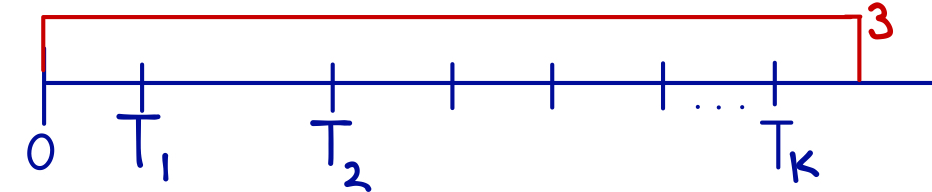
\includegraphics[height=1.4cm, width=12cm]{HW6/P2.jpeg}$$
    
    
    \item $P(N(2)=k\;|\; T_3 > 4)$
    $$=\frac{P(N(2)=k\;|\;N(4)<3)}{P(N(4)<3)}=\frac{P(N(2)=k)\cdotP(N(2)<3-k)}{P(N(4)<3)}$$
    $$=\frac{\left(e^{-2\lambda}\frac{(2\lambda)^k}{k!}\right)
    \left(\sum\limits_{k=0}^{3-k-1}P(N(2)=3-k)\right)}
    {\sum\limits_{k=0}^{2} P(N(4)=k)}
    =\frac{\left(e^{-2\lambda}\frac{(2\lambda)^k}{k!}\right)
    \left(\sum\limits_{k=0}^{3-k-1}e^{-2\lambda}\frac{(2\lambda)^k}{k!}\right)}
    {\sum\limits_{k=0}^{2} e^{-4\lambda}\frac{(4\lambda)^k}{k!}}
    $$
    
    \vspace{2\baselineskip}
    \item $P(T_2\le 3\;|\; N(4)=5).$ Explain how your answer can be expressed in terms of a certain binomial probability mass function.
    \begin{align}
        P(T_2\le 3\;|\; N(4)=5)&=\frac{\sum\limits_{n=2}^5\left(\cancel{e^{-3\lambda}}\cdot \frac{(3\cancel{\lambda})^n}{n!}\right)
       \left(\cancel{e^{-\lambda}}\cdot \frac{\cancel{\lambda}^{5-n}}{(5-n)!}\right)}{\cancel{e^{-4\lambda}}\cdot\frac{(4\cancel{\lambda})^5}{(5-n)!}} \nonumber \\
       &=\frac{5!}{4^5}\left[
       \left(\frac{3^2}{2!\cdot 3!}\right)+\left(\frac{3^3}{3!\cdot 2!}\right)
       +\left(\frac{3^4}{4!\cdot 1!}\right)+\left(\frac{3^5}{5!\cdot 0!}\right)
       \right] \nonumber \\
       &= \sum\limits_{n=2}^5 \binom{5}{n}\left(\frac{3}{4}\right)^n\cdot \left(\frac{1}{4}\right)^{5-n} \nonumber
    \end{align}
    
    
   
\end{enumerate}

\newpage
{\bf 2.36 } Customers arrive at an automated teller machine at the times of a Poisson process with rate of 10 per hour. Suppose that the amount of money withdrawn on each transaction has a mean of \$30 and a standard deviation of \$20. Find the mean and standard deviation of the total withdrawals in 8 hours.

\vspace{1\baselineskip}
Given the time $[0,t]$, let 
\begin{itemize}
    \item $Y_n$ be the amount of $n^{th}$ withdrawal
    \item $W(t)$ be total amount withdrawn: $W(t)=Y_1+Y_2+...+Y_n$
    \item $N(t)$ be the number of customers
    \item $\mu$ be the mean and $\sigma$ be the standard deviation
\end{itemize}
Then we can formulate $$W(t)=\sum\limits_{i=1}^{N(t)} Y_i$$

For the mean,
$$E[W(t)] 
= \sum\limits_{n=0}^{N(t)} \underbrace{E\left[W(t)\;|\;N(t)=n\right]}_{nE[Y_i]=nE[Y]} \cdot \underbrace{P(N(t)=n)}_{e^{-t\lambda}\frac{(t\lambda)^{n}}{n!}}$$
$$nE[Y_i]\cdot e^{-t\lambda}\frac{(t\lambda)}{n}\cdot \underbrace{\sum\limits_{n=1}^{N(t)}\frac{(t\lambda)^{n-1}}{(n-1)!}}_{\text{Taylor Expansion: }e^{t\lambda}}
=\cancel{n}E[Y_i]\cdot \cancel{e^{-t\lambda}}\frac{(t\lambda)}{\cancel{n}}\cdot \cancel{e^{t\lambda}}=t\lambda \mu$$
$$=8\cdot10\cdot \$30 = \$2,400 $$

\vspace{2\baselineskip}
For the standard deviation, $\sigma = \sqrt{Var[{W(t)}]}= \sqrt{E[W^2(t)]-E^2[W(t)]}$
$$E[W^2(t)]= \sum\limits_{n=0}^{N(t)} E\underbrace{\left[W^2(t)\;|\;N(t)=n\right]}_{(Y_1+...+Y_n)^2} \cdot \underbrace{P(N(t)=n)}_{e^{-t\lambda}\frac{(t\lambda)^{n}}{n!}}$$
$$E[W^2(t)\;|\;N(t)=n] = \underbrace{E[Y_1^2]+E[Y_2^2]+\ldots+ E[Y_n^2]}_{n\text{ terms}}
+2(\underbrace{E[Y_1]E[Y_2]+E[Y_1]E[Y_3]+E[Y_2]E[Y_3]+\ldots)}_{\frac{n(n-1)}{2}\text{ terms}}$$

\vspace{1\baselineskip}
Since this is $i.i.d,\; E[Y_1]=E[Y_2]=...=E[Y_n]$
$$E[W^2(t)\;|\;N(t)=n]=n\cdot E[Y^2] + n(n-1) E^2[Y]$$

\vspace{1\baselineskip}
Remind that $E[Y^2] = \sigma^2 +\mu^2$. Then
$$E[W^2(t)\;|\;N(t)=n]=n(\sigma^2+\mu^2) + n(n-1)\cdot \mu^2 = n\sigma^2+n^2\mu^2$$

$$E[W^2(t)] 
= \sum\limits_{n=0}^{N(t)} (n\sigma^2+n^2\mu^2)\cdot e^{-t\lambda}\frac{(t\lambda)^{n}}{n!}
=\sigma^2 \underbrace{\sum\limits_{n=0}^{N(t)} n e^{-t\lambda}\frac{(t\lambda)^{n}}{n!}}_{Expectation}
+\mu^2 \underbrace{\sum\limits_{n=0}^{N(t)} n^2 e^{-t\lambda}\frac{(t\lambda)^{n}}{n!}}_{Expectation\; of\; square}$$
$$=\sigma^2 E[N(t)] + \mu^2 E[N^2(t)]$$

Hence
$$Var[W(t)] = E[W^2(t)] - E^2[W(t)] = \sigma^2 E[N(t)] + \mu^2 E[N^2(t)] - (\mu\underbrace{\lambda t)^2}_{E^2[N(t)]}$$

Note that by Lemma 2.2 on Durrett, $N(t)$ has a Poisson distribution with means $\lambda t$, 

$$\sigma^2 E[N(t)] + \mu^2 \underbrace{(E[N^2(t)] - E^2[N(t)])}_{Var(N(t)}
$$
We also know that mean is equal to variance for Poisson distribution. Hence

$$Var[W(t)]=\sigma^2 E[N(t)] + \mu^2 E[N(t)] = (\sigma^2 + \mu^2)\lambda t = (\$20^2 + \$30^2)10\cdot 8 = 104,000$$

\vspace{1\baselineskip}
Thus the standard deviation is $\sqrt{104,000}$.

\newpage
{\bf 2.38 } Let $S_t$ be the price of stock at time t and suppose that at times of a Poisson process with rate $\lambda$ the price is multiplied by a random variable $X_i > 0$ with mean $\mu$ and variance $\sigma^2$. That is $$S_t = S_0 \prod_{i=1}^{N(t)} X_i$$ where the product is 1 if $N(t)=0$. Find $ES(t)$ and Var$S(t)$. \\

\begin{align}
   E[S_t] &= E\left[S_0 \prod_{i=1}^{N(t)} X_i\right] =\nonumber S_0\prod_{i=1}^{N(t)} E[X_i] = S_0 \mu^{N(t)} =S_0 \sum\limits_{k=0}^\infty E[X_i\;|\;N(t)=k]\cdot P[N(t)=k]\\ \nonumber
   &=S_0 \sum\limits_{k=0}^\infty \mu^k e^{-\lambda t} \cdot \frac{(\lambda t)^k}{k!}
    =S_0 e^{-\lambda t} \underbrace{\sum\limits_{k=0}^\infty \frac{(\mu\lambda t)^k}{k!}}_{e^{\mu\lambda t}}
    =S_0e^{\lambda t(\mu -1)} 
\end{align}

\begin{align}
    Var[S_t] &= E[S_t^2] - E^2[S_t] = E\left[S_0^2 \prod_{i=1}^{N(t)} X_i^2\right] - (S_0e^{\lambda t(\mu -1)})^2  \nonumber \\
    &= S_0^2\prod_{i=1}^{N(t)} E[X_i^2] - S_0^2e^{2(\mu-1)\lambda t}
    = S_0^2\prod_{i=1}^{N(t)} (\sigma^2 + \mu^2) - S_0^2e^{2(\mu-1)\lambda t}\nonumber \\
    &=S_0^2 (\sigma^2 + \mu^2)^{N(t)} - S_0^2e^{2(\mu-1)\lambda t} 
    = S_0^2\sum\limits_{k=0}^\infty (\sigma^2 + \mu^2)^k\cdot \left(
    e^{-t\lambda}\cdot \frac{(t\lambda)^k}{k!}\right) - S_0^2e^{2(\mu-1)t\lambda}\nonumber \\
    &=S_0^2e^{-t\lambda}\sum\limits_{k=0}^\infty \frac{((\mu^2+\sigma^2)t\lambda)^k}{k!}- S_0^2e^{2(\mu-1)}
    =S_0^2e^{-t\lambda} e^{(\mu^2+\sigma^2)t\lambda}- S_0^2e^{2(\mu-1)t\lambda}\nonumber\\
    &=S_0^2(e^{t\lambda((\mu^2+\sigma^2)-1)}-e^{2(\mu-1)t\lambda} )\nonumber
\end{align}

\vspace{2.5\baselineskip}
{\bf 2.44 }Ellen catches fish at times of a Poisson process with rate 2 per hour. 40\% of the fish are salmon, while 60\% of the fish are trout. What is the probability she will catch exactly 1 salmon and 2 trout if she fishes for 2.5 hours?

\vspace{1\baselineskip}
Let $N_s(t)$ be the number of salmon Ellen catches for time $t$ with rate $2\times 40\% = 0.8$ and $N_t$ be that of trout with rate $2\times 60\% = 1.2$. Then we can formulate the probability Ellen will catch exactly 1 salmon and 2 trout for 2.5 hours as below.

$$P(N_s(2.5)=1,\;N_t(2.5)=2) = P(N_s(2.5)=1)\cdot P(N_t(2.5)=2)$$
$$\left(e^{-2.5\times 0.8}\frac{(-2.5\times 0.8)^2}{2!}\right)\cdot
\left(e^{-2.5\times 1.2}\frac{(-2.5\times 1.2)^1}{1!}\right) 
=9e^{-5}$$

\newpage
%\vspace{1\baselineskip}
{\bf 2.48 } When a power surge occurs on an electrical line, it can damage a computer without a surge protector. There are three types of surges: “small” surges occur at rate 8 per day and damage a computer with probability 0.001; “medium” surges occur at rate 1 per day and will damage a computer with probability 0.01; “large” surges occur at rate 1 per month and damage a computer with probability 0.1. Assume that months are 30 days.
\begin{enumerate}[label=(\alph*)]
    \item What is the expected number of power surges per month?
    $$\underbrace{8\times 30}_{\text{Small Surges}} + \underbrace{1\times 30}_{\text{Medium Surges}} + \underbrace{1}_{\text{Large Surges}} = 271$$
    
    \item What is the expected number of computer damaging power surges per month?
    
    $$8\times 30\times 0.001 + 1\times 30\times 0.01 + 1\times 0.1 = 0.64$$
    \item What is the probability a computer will not be damaged in one month?
    $t=1$ since 30-days is the unit time for this question.
    \begin{itemize}
        \item Small Surge: $\lambda = 0.001\times (8\cdot 30)$=0.24
        $$P(\text{No damage due to small surge})=P(N(t)=0) = e^{-0.24}\cdot \frac{0.24^0}{0!}=e^{-0.24}$$
        
        \item Medium Surge: $\lambda = 0.01\times (1\cdot 30) = 0.3$
        $$P(\text{No damage due to medium surge})=P(N(t)=0) = e^{-0.3}\cdot \frac{0.3^0}{0!}=e^{-0.3}$$
        
        \item Large Surge: $\lambda = 0.1\times 1 = 0.1$
        $$P(\text{No damage due to large surge})=P(N(t)=0) = e^{-0.1}\cdot \frac{0.1^0}{0!}=e^{-0.1}$$
    \end{itemize}
    
    Hence the probability a computer will not be damaged in one month is
    $$e^{-0.24}\times e^{-0.3}\times e^{-0.1}=e^{-0.64}$$
    
    \item What is the probability that the first computer damaging surge is a small one?
    $$\frac{e^{-0.24}}{e^{-0.64}}$$
    
\end{enumerate}

\newpage
{\bf 2.49 }Wayne Gretsky scored a Poisson mean 6 number of points per game. 60\% of these were goals and 40\% were assists (each is worth one point). Suppose he is paid a bonus of 3K for a goal and 1K for an assist.
\begin{enumerate}[label=(\alph*)]
    \item Find the mean and standard deviation for the total revenue he earns per game.\\
    
    Let $G_i$ be the number of score he made and $A_i$ be that of assist per game. 
    $$\text{Average Goals per game: }0.6\cdot 6 = 3.6 \qquad 
    \text{Average Assists per game: }0.4\cdot 6 = 2.4$$
    $$E[Goals] = \underbrace{E[N]}_{3000}\cdot \underbrace{E[G_i]}_{3.6}= 10800 \qquad
    E[Assists] = \underbrace{E[N]}_{1000}\cdot \underbrace{E[A_i]}_{2.4}= 2400    $$
    
    Now let $X_i$ be the points he gain on $i^{th}$ game and $P= X_1+X_2+...+X_n$. Then
    $$E[P] = 10800+2400 = 13200$$
    $$Var[P] = 3000^2\cdot 3.6+1000^2\cdot 2.4$$

    \item What is the probability that he has 4 goals and 2 assists in one game?
    $$P(\text{Poisson}(1)=4)\cdot P(\text{Poisson}(1)=2) 
    = \left(e^{-3.6}\cdot \frac{3.6^4}{4!}\right) \cdot \left(e^{-2.4}\cdot \frac{2.4^2}{2!}\right)$$
    \item Conditional on the fact that he had 6 points in a game, what is the probability he had 4 in the first half?
    $$P(N(1/2)=4\;|\;N(1)=6) = \binom{6}{4}\cdot \left(\frac{1}{ 2}\right)^2\cdot \left(\frac{1}{2}\right)^4 = 0.234375
    $$
\end{enumerate}

\newpage
{\bf 2.51 }Two copy editors read a 300-page manuscript. The first found 100 typos, the second found 120, and their lists contain 80 errors in common. Suppose that the author’s typos follow a Poisson process with some unknown rate  per page, while the two copy editors catch errors with unknown probabilities of success $p_1$ and $p_2$. Let $X_0$ be the number of typos that neither found. Let $X_1$ and $X_2$ be the number of typos found only by 1 or only by 2, and let $X_3$ be the number of typos found by both.
\begin{enumerate}[label=(\alph*)]
    \item Find the joint distribution of $(X_0,X_1,X_2,X_3)$.\\
    
    Rates for those independent Poisson process are
    \begin{tasks}[label](2)
        \task $X_0:\; (1-p_1)(1-p_2)\lambda$
        \task $X_1:\; p_1(1-p_2)\lambda$
        \task $X_2:\; p_2(1-p_1)\lambda$
        \task $X_3:\; p_1p_2$
    \end{tasks}
    
    $$P(X_0=n_0,\;X_1=n_1,\;X_2=n_2,\;X_3=n_3)
    =e^{-300(1-p_1)(1-p_2)\lambda}\frac{(300(1-p_1)(1-p_2)\lambda)^{n_0}}{n_0!}\times$$
    $$
    e^{-300p_1(1-p_2)\lambda}\frac{(300p_1(1-p_2)\lambda)^{n_1}}{n_1!}\times e^{-300p_2(1-p_1)\lambda}\frac{(300p_2(1-p_1)\lambda)^{n_2}}{n_2!}\times
    e^{-300p_1p_2\lambda}\frac{(300p_1p_2)^{n_3}}{n_3!} 
    $$
    
    \vspace{1\baselineskip}
    Since $((1-p_1)((1-p_2)+p_2)+p_1((1-p_2)+p_2) = 1$,\\
    
    $P(X_0=n_0,\;X_1=n_1,\;X_2=n_2,\;X_3=n_3)$
    $$=e^{-300\lambda}
    300\lambda^{n_0+n_1+n_2+n_3}\times \frac{
    (1-p_1)(1-p_2)^{n_0}+(p_1(1-p_2))^{n_1} + p_2(1-p_1)^{n_2} + (p_1p_2)^{n_3}
    }{n_0!n_1!n_2!n_3!}$$
    \item Use the answer to (a) to find an estimates of $p_1,p_2$ and then of the number of undiscovered typos.
    
    \begin{itemize}[label={}]
        \item $E[X_1]=300\cdot \lambda p_1(1-p_2)=20$
        \item $E[X_2]=300\cdot \lambda p_2(1-p_1)=40$
        \item $E[X_3]=300\cdot \lambda p_1p_2=80$
    \end{itemize}
    $$\frac{E[X_2]}{E[X_3]} = \frac{1-p_1}{p_1} = \frac{1}{p_1}-1 = \frac{1}{2} \;\;\Leftrightarrow\;\;p_1 = \frac{2}{3}$$
    $$2\cdot \frac{2}{3}(1-p_2) = \frac{1}{3}\cdot p_2\;\;\Leftrightarrow\;\;
    \frac{1}{p_2} - 1 = \frac{1}{3}\cdot \frac{3}{4} = \frac{1}{4} \;\;\Leftrightarrow\;\;p_2=\frac{4}{5}$$
    $$300\cdot \lambda \frac{2}{3}\cdot \frac{4}{5} = 160\lambda = 80\;\;\Leftrightarrow\;\;\lambda = \frac{1}{2}$$
    Hence
    $$E[X_0] = 300\cdot \frac{1}{2}\cdot\frac{1}{3}\cdot \frac{1}{5} = 10$$
\end{enumerate}
\end{document}